\documentclass{beamer}
\usepackage{amsthm}
\usepackage{times}
\usepackage{graphicx}
\usefonttheme{professionalfonts}
\usetheme{Boadilla}
%\usecolortheme{sidebartab}
\title{Interbrain data analysis}
%\subtitle{L'equazione di Fisher}
\author[F. Bernardi]{\textbf{Fabrizio Bernardi}} \medskip
%\titlegraphic{
\includegraphics[scale=.1]{Logo_Politecnico_Milano.jpg}}
%\titlegraphic{
\includegraphics[scale=.3]{Logo_IIT.png}}





\date[26/10/2021]{26/10/2021}


\begin{document}
	
	
		\begin{frame}
	\maketitle
	
	\begin{minipage}{\linewidth}
		\centering
		\begin{minipage}{0.45\linewidth}
			\begin{figure}[H]
				
\includegraphics[width=\linewidth]{Logo_IIT.png}
				
			\end{figure}
		\end{minipage}
		\hspace{0.05\linewidth}
		\begin{minipage}{0.45\linewidth}
			\begin{figure}[H]
				
\includegraphics[width=\linewidth]{Logo_Politecnico_Milano.jpg}
				
			\end{figure}
		\end{minipage}
	\end{minipage}
\end{frame}

\begin{frame}
\frametitle{The experiment}


	
\begin{figure}[H]
	\begin{center}
		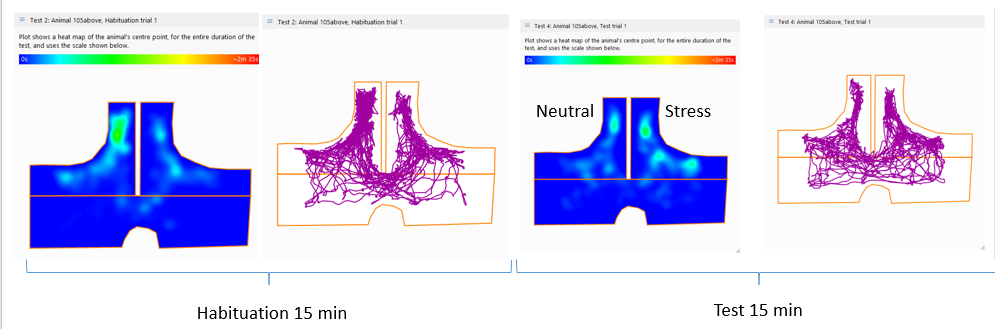
\includegraphics[scale=.40]{overview_experiment.png} 
	\end{center} 
\end{figure}


\begin{itemize}
	\item Observer, neutral and stressed mice in an arena
	
	\item 5 minutes of home cage, 15 of habituation, 15 of test
\end{itemize}

\end{frame}	
	
\begin{frame}
\frametitle{The dataset}


\begin{itemize}
	\item Observer, neutral and stressed neuronal activities over time
	
	\item Recording of observer's position during habituation and test
	
	\item Recording of reciprocal sniffing during test
	
	
\end{itemize}
\end{frame}	
	
	
	
	\begin{frame}
	\frametitle{Goals}
	
	
	\begin{itemize}
		\item Study single neuronal activity and aggregate activity of 3 mice
		
		\item Look for relationship between activity and interactions between mice
		
		\item Investigate the presence of synchronized activity between mice, studying relationship with mice interactions
		
		
		
		
	\end{itemize}
\end{frame}	



\begin{frame}
\frametitle{Preparing the dataset}

First technical steps consisted in:

\begin{itemize}
	\item Excluding the neurons marked as \textit{rejected} from Inscopix and separate the dataset for the three mice and the three stages
	
	\item Adapting the times  based on the A keyboard information in the sniff file
	
	\item Final time adapting which aligns the three time intervals and considers the same time points (using linear interpolation)
	
	\item z-score, min-max and homecage normalizations are provided
	
	
	
\end{itemize}
\end{frame}	


\begin{frame}
\frametitle{Single neuron activity}

\begin{figure}[H]
	\begin{center}
		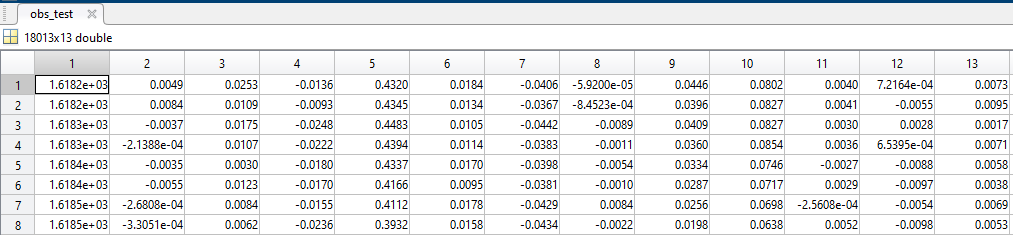
\includegraphics[scale=.45]{single_neuron_data.png} 
	\end{center} 
\end{figure}


\begin{figure}[H]
	\begin{center}
		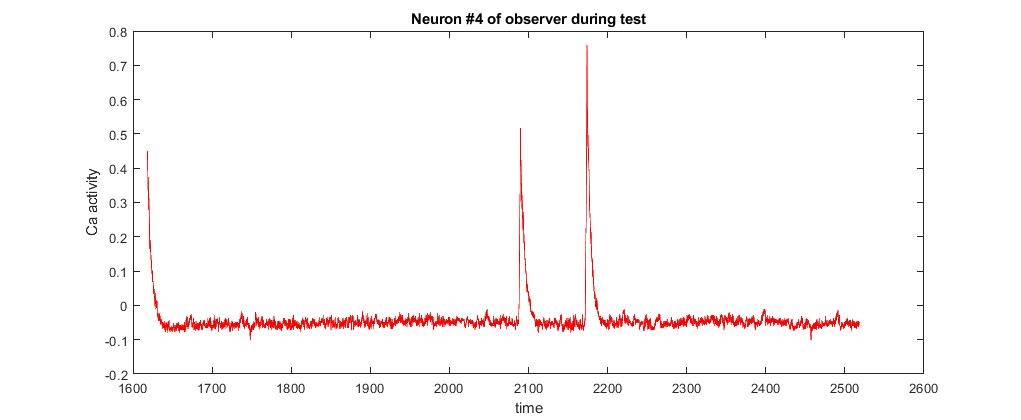
\includegraphics[scale=.30]{neuron4.jpg} 
	\end{center} 
\end{figure}

\end{frame}	


\begin{frame}
\frametitle{Mice overall activity}

The overall activity for one mouse is computed as the average of all its neuronal activities at each time step

\vspace{1 cm}

	\begin{minipage}{\linewidth}
	\centering
	\begin{minipage}{0.20\linewidth}
		\begin{figure}[H]
			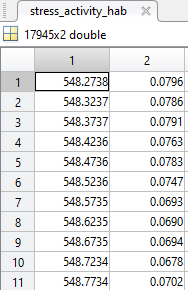
\includegraphics[scale=.50]{overall_data.png}
			
		\end{figure}
	\end{minipage}
	\hspace{0.01 cm}
	\begin{minipage}{0.70\linewidth}
		\begin{figure}[H]
			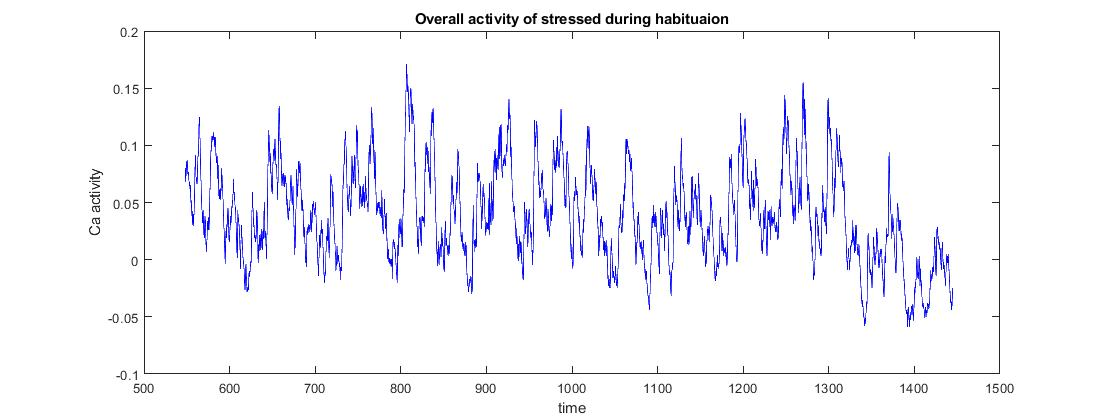
\includegraphics[scale=.25]{overall_activity.jpg}
			
		\end{figure}
	\end{minipage}
\end{minipage}

\end{frame}	



\begin{frame}
\frametitle{Activity detection}

How do we establish if a neuron is active or not?

\begin{itemize}
	\item Standard way: all above a treshold line ( $ y = \mu + 2\sigma$) is active and vieversa
	
	\item \textbf{MAD} algorithm (Inscopix manual): the treshold line varies with the signal
	
	
	
	
\end{itemize}

\begin{figure}[H]
	\hspace*{-1cm}  
		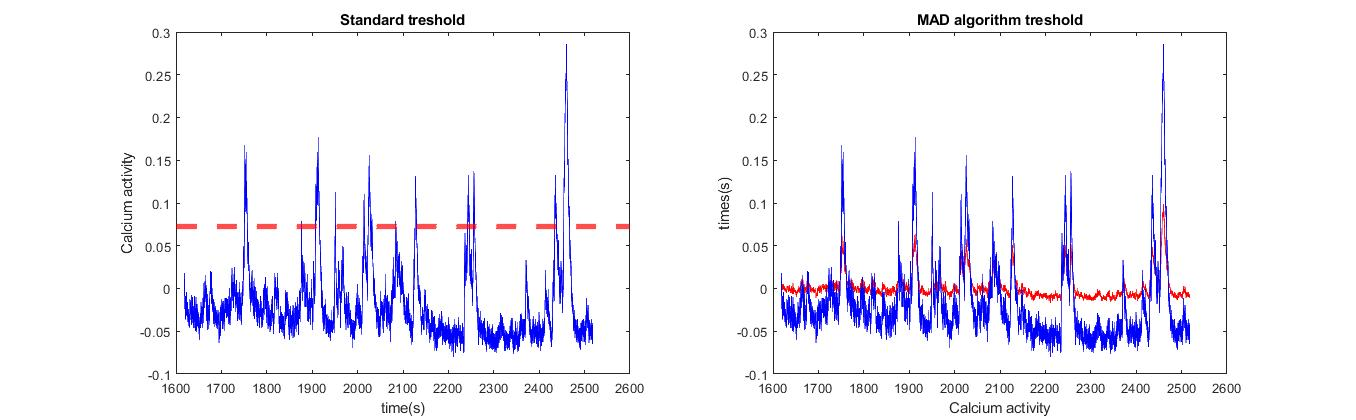
\includegraphics[scale=.30]{treshold.jpg} 
	 
\end{figure}


\end{frame}	


\begin{frame}
\frametitle{Other features (1)}

	
	


\begin{figure}[H]
	\begin{center}
		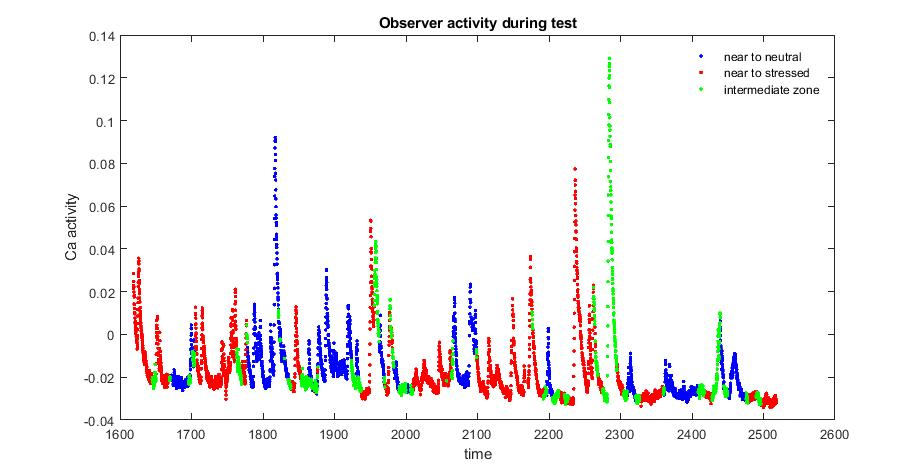
\includegraphics[scale=.40]{zone_plot.jpg} 
	\end{center}  
	
	
\end{figure}


\end{frame}	


\begin{frame}
\frametitle{Other features (2)}





\begin{figure}[H]
	\begin{center}
		\hspace*{-1cm}
		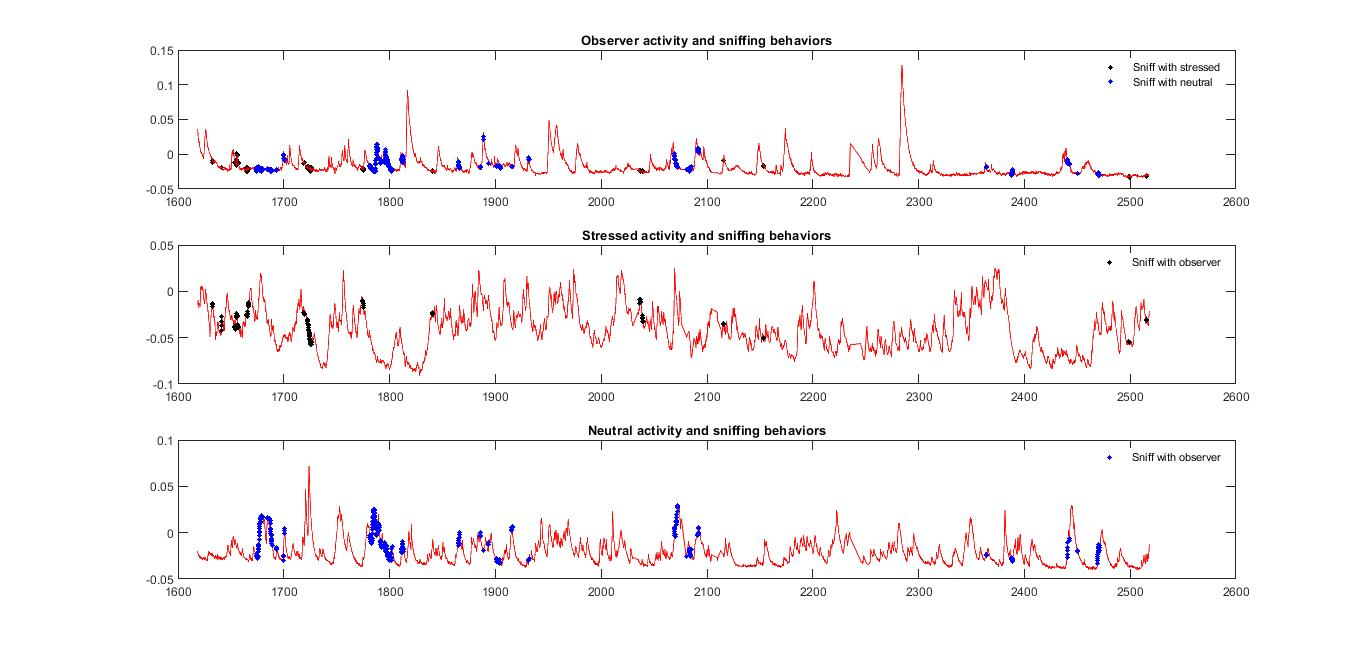
\includegraphics[scale=.30]{sniff_plot.jpg} 
	\end{center}  
	
	
\end{figure}


\end{frame}	


\begin{frame}
\frametitle{Other features (3)}





\begin{figure}[H]
	\begin{center}
		\hspace*{-1cm}
		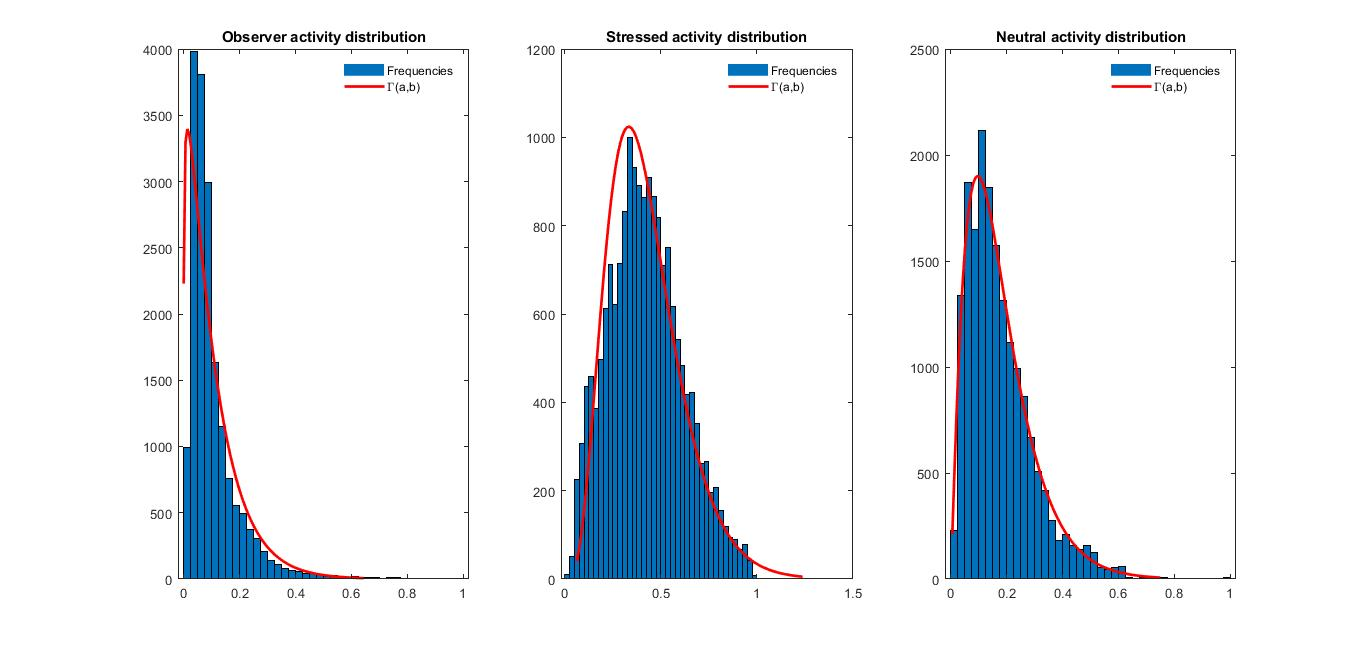
\includegraphics[scale=.30]{hist.jpg} 
	\end{center}  
	
	
\end{figure}


\end{frame}	

\begin{frame}
\frametitle{First conclusions on single activity analysis}

\begin{itemize}
	\item No particular relationship between neuronal activity peaks and mice vicinity
	
	\item Sniffing in observer seems to be usually followed by activity peaks
	
	\item The mean activity of neurons is higher in stressed mouse respect to the other two
	
	\item More data should be necessary to infer conclusions
	
	
	
	
\end{itemize}

	

\end{frame}	




\begin{frame}
\frametitle{Correlation indicators}


\begin{enumerate}
	\item \textbf{Pearson correlation}: it tells how \textit{linearly} correlated two random quantities are
	
	$$ Corr_P(X,Y) = \frac{Cov(X,Y)}{\sigma_X \sigma_Y} $$
	
	\item \textbf{Cross correlation}: similarity measure for signals, given as function of the reciprocal delay
	
	$$  Corr_C(X,Y)  = X \star Y (t) = X(-t)*Y(t) = \int_{-\infty}^{\infty}X(t-\tau)Y(t) dt $$
	
	$$  Corr_C(X,Y)  = X \star Y (m) = \sum_{n=0}^{N-m-1} X_{n+m}Y_n  $$
	
	
	
	
	
	
	
	
\end{enumerate}





\end{frame}	


\begin{frame}
\frametitle{Correlation indicators}


\begin{itemize}
	\item Pearson correlation may not be the best choice for a strongly nonlinear signal (but it may still have some significance as term of comparison between two scenarios)
	
	\item Cross correlation, on the other hand, seems the best way to quantify similarity between two signals
	
\vspace{1 cm}
		\begin{minipage}{\linewidth}
		\centering
		\begin{minipage}{0.20\linewidth}
			\begin{figure}[H]
				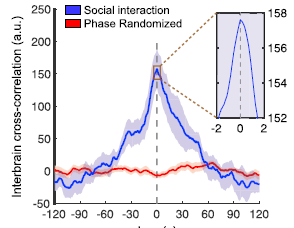
\includegraphics[scale=.70]{kingsbury1.png}
				
			\end{figure}
		\end{minipage}
		\hspace{0.7 cm}
		\begin{minipage}{0.70\linewidth}
			\begin{figure}[H]
				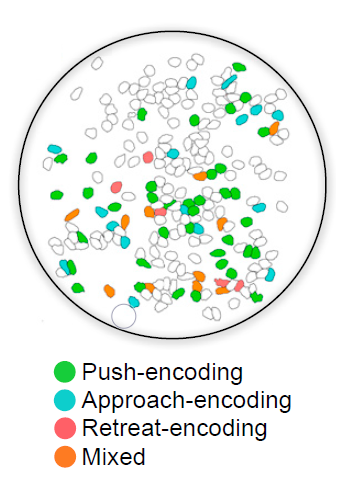
\includegraphics[scale=.70]{kingsbury2.png}
				
			\end{figure}
		\end{minipage}
	\end{minipage}
		
	
	
\end{itemize}





\end{frame}	




\begin{frame}
\frametitle{Activities synchronization: observer vs stressed}





\begin{figure}[H]
	\begin{center}
		\hspace*{-1cm}
		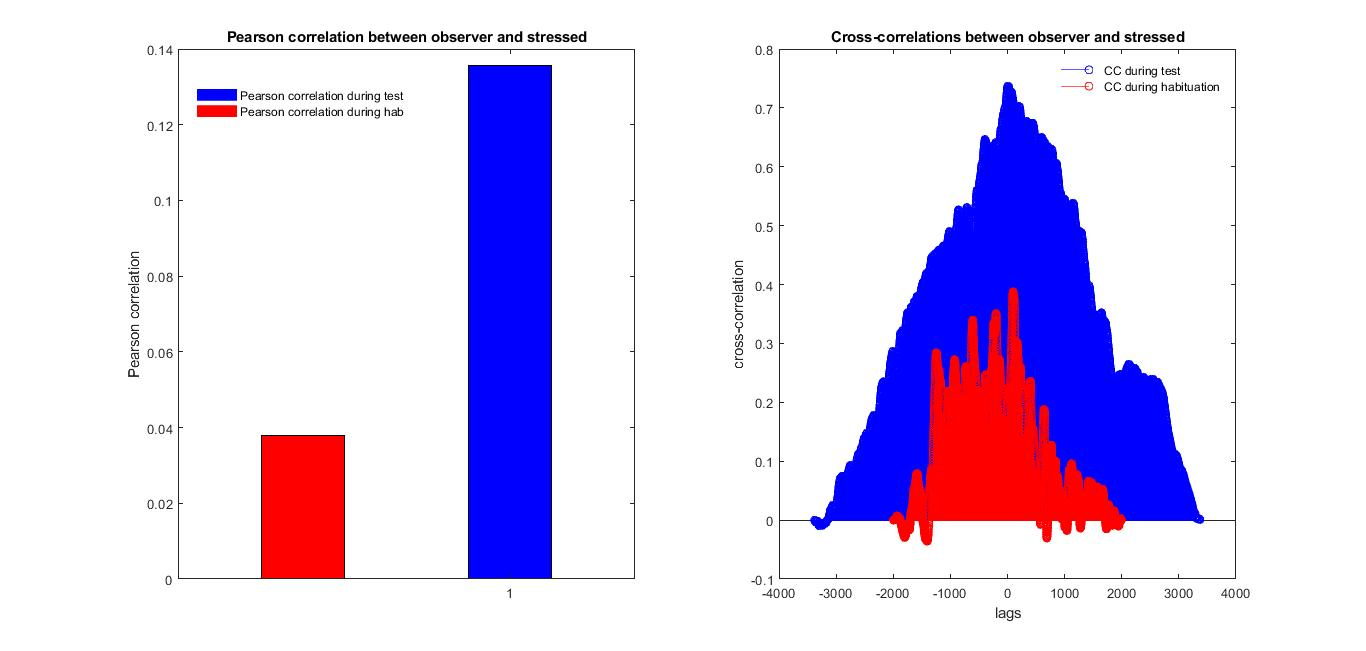
\includegraphics[scale=.30]{obs_stress_sync.jpg} 
	\end{center}  
	
	
\end{figure}


\end{frame}	

\begin{frame}
\frametitle{Activities synchronization: observer vs neutral}





\begin{figure}[H]
	\begin{center}
		\hspace*{-1cm}
		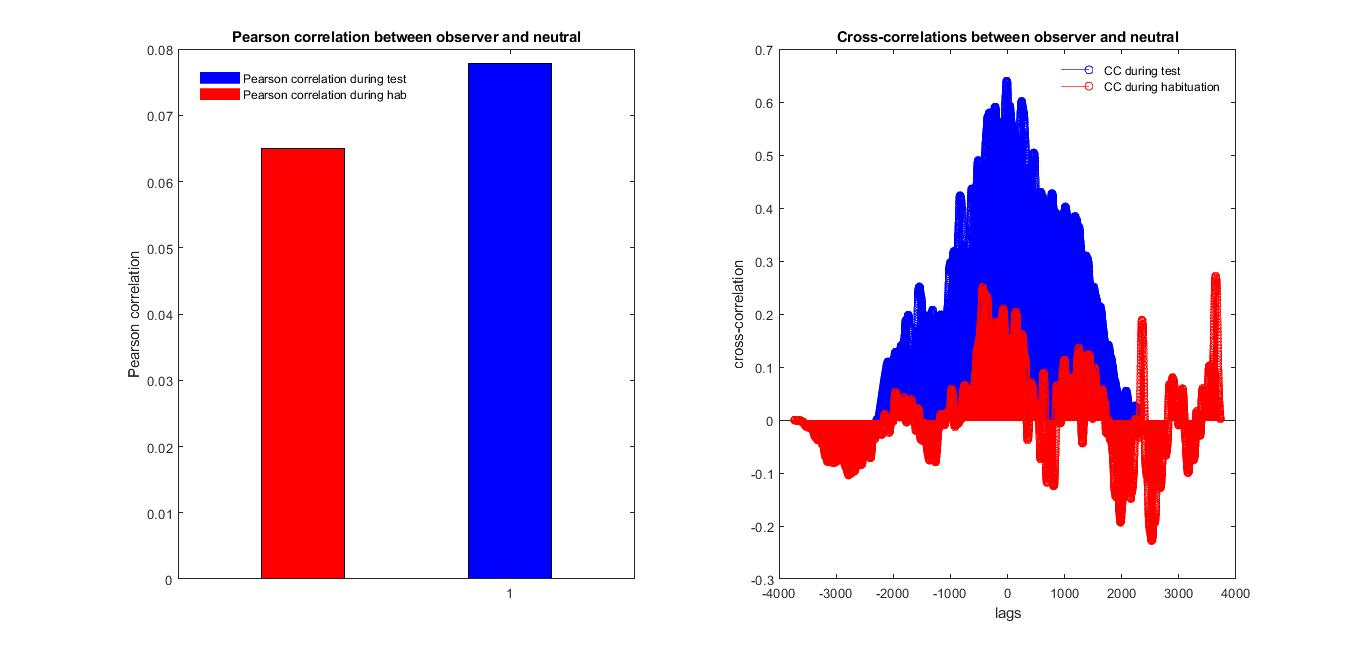
\includegraphics[scale=.30]{obs_neutral_sync.jpg} 
	\end{center}  
	
	
\end{figure}


\end{frame}	


\begin{frame}
\frametitle{Activities synchronization: distant mice}





\begin{figure}[H]
	\begin{center}
		\hspace*{-1cm}
		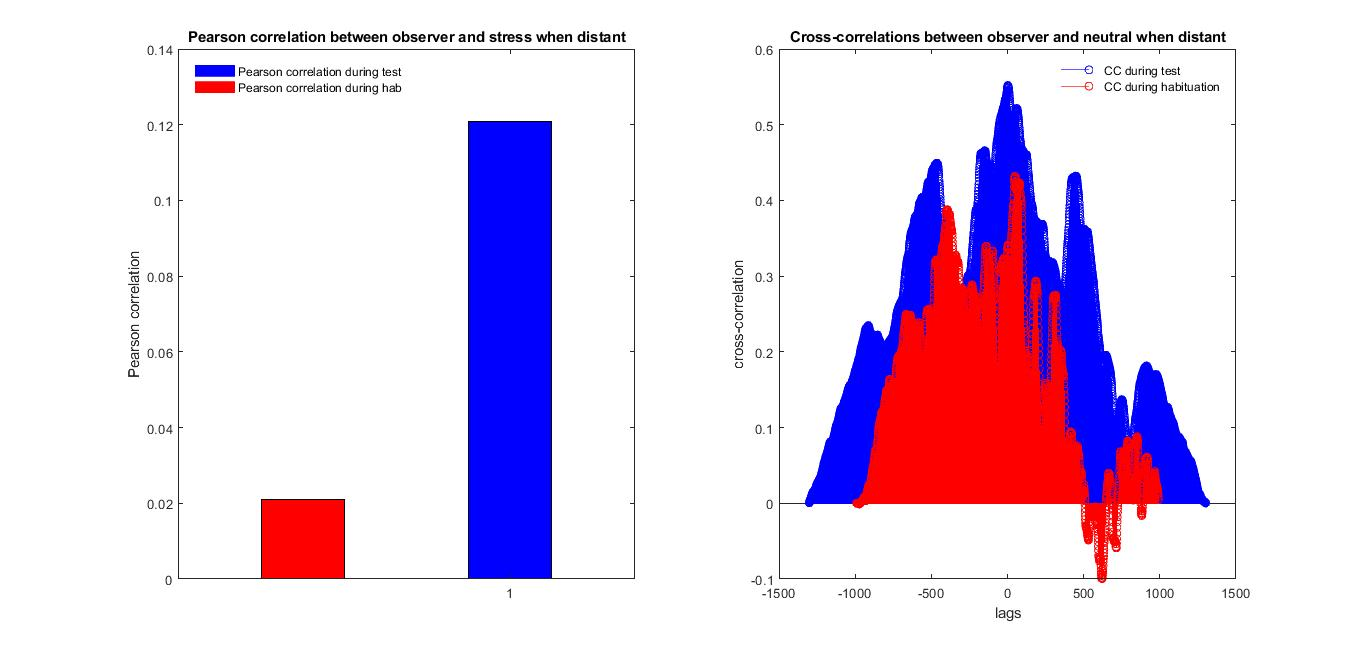
\includegraphics[scale=.30]{distant_sync.jpg} 
	\end{center}  
	
	
\end{figure}


\end{frame}	


\begin{frame}
\frametitle{Activities synchronization: reciprocal sniffing}





\begin{figure}[H]
	\begin{center}
		\hspace*{-1cm}
		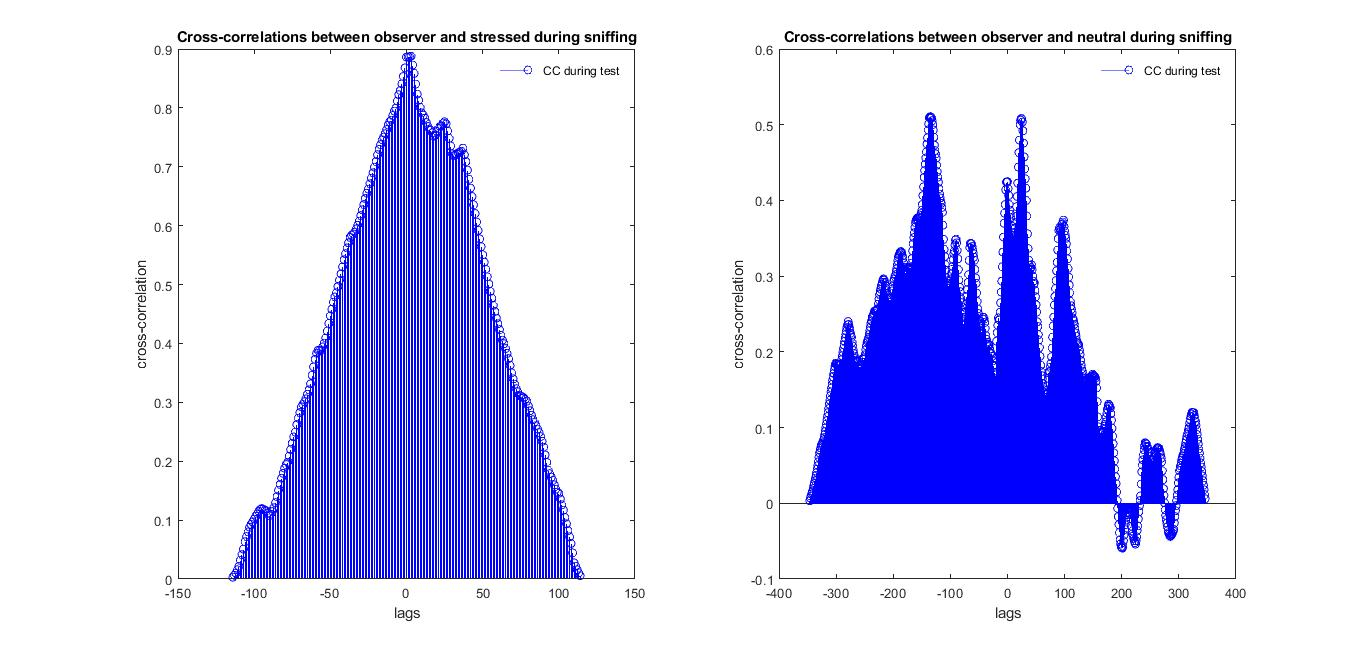
\includegraphics[scale=.30]{sniff_corr.jpg} 
	\end{center}  
	
	
\end{figure}


\end{frame}	

\begin{frame}
\frametitle{Overall correlation change}



\begin{figure}[H]
	\begin{center}
		\hspace*{-1cm}
		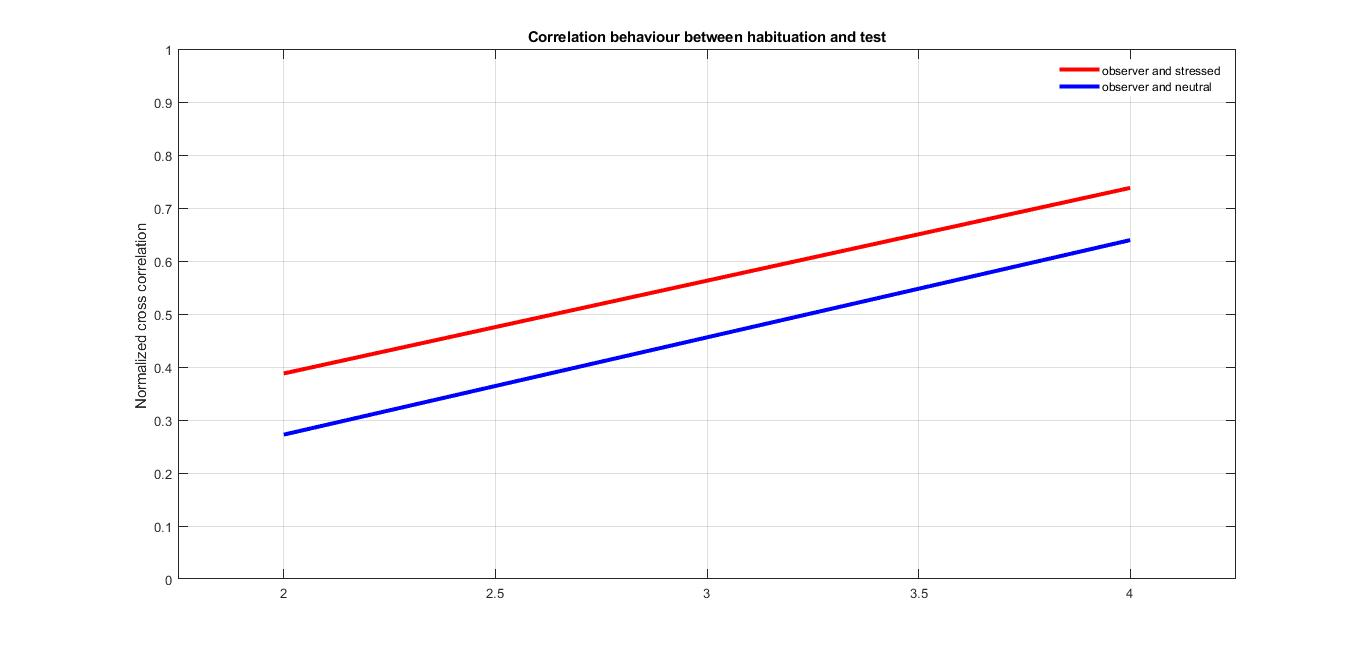
\includegraphics[scale=.30]{corr_line.jpg} 
	\end{center}  
	
	
\end{figure}

\end{frame}

\begin{frame}
\frametitle{Conclusions on the overall correlation analysis}



\begin{itemize}
	
	\item The correlation between the observer and the stressed mice appears strong and in counterposition with the habituation phase
	
	\item Altough less marked than the previous one, also the correlation between observer and neutral mice is definitely higher during the test than the habituation
	
	\item This difference is less evident when the two mice are not in contact
	
	\item When sniffing, the correlation between observer and stressed is the highest recorded
	
	
	
\end{itemize}

\end{frame}	


\begin{frame}
\frametitle{Neuron pairs synchronization: observer vs stressed during test (1)}





\begin{figure}[H]
	\begin{center}
		\hspace*{-1cm}
		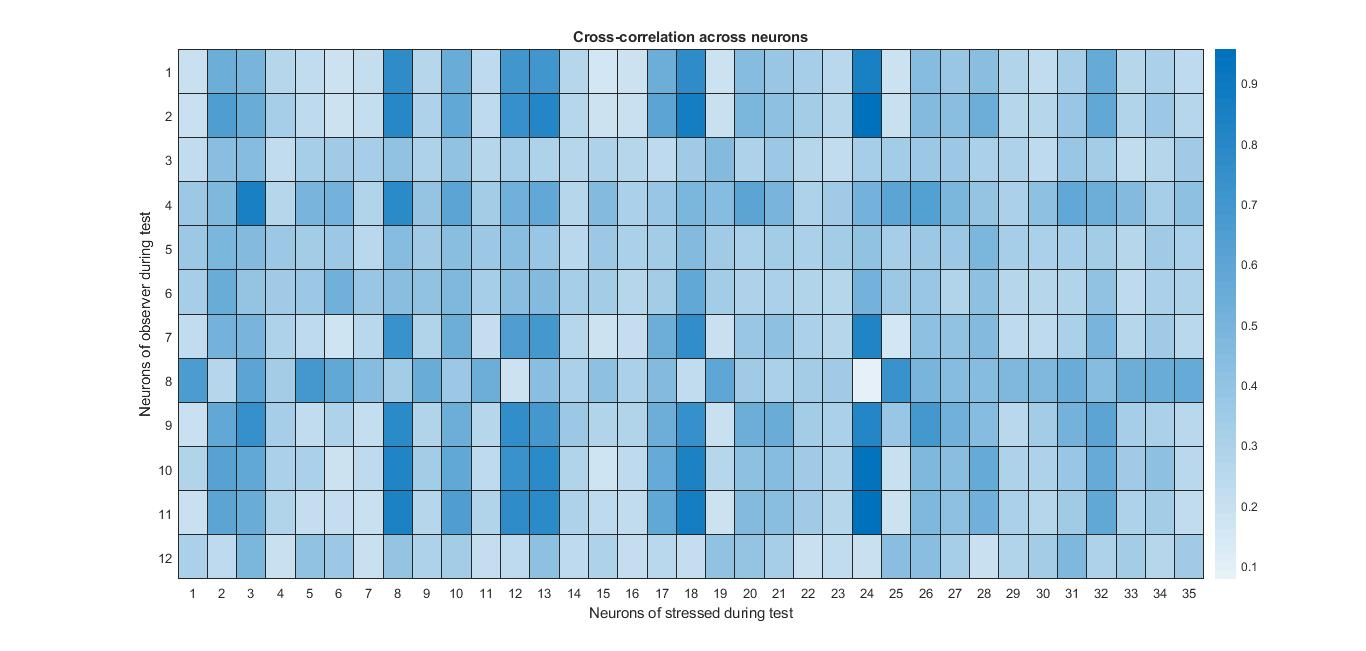
\includegraphics[scale=.30]{cc_heatmap.jpg} 
	\end{center}  
	
	
\end{figure}


\end{frame}	




\begin{frame}
\frametitle{Neuron pairs synchronization: observer vs stressed during test (2)}


Fraction of pairs showing correlation = $11.43 \%$


\begin{figure}[H]
	\begin{center}
		\hspace*{-1cm}
		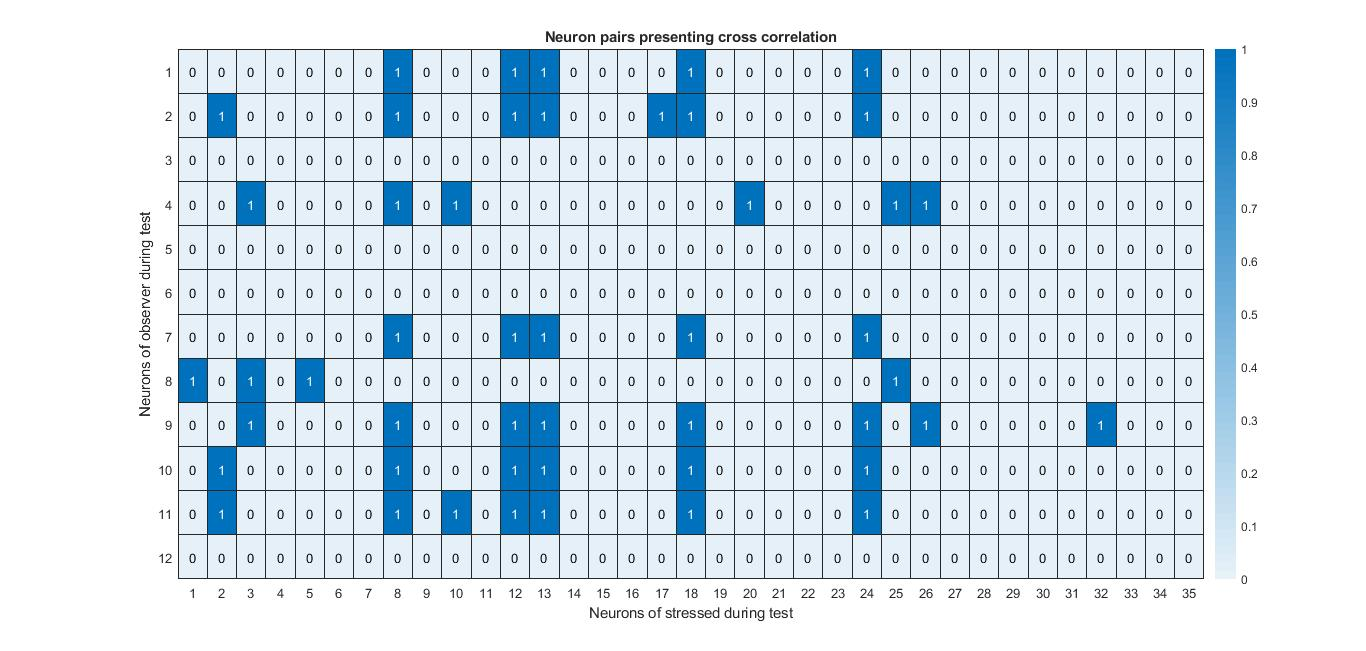
\includegraphics[scale=.30]{cc_active.jpg} 
	\end{center}  
	
	
\end{figure}


\end{frame}	


\begin{frame}
\frametitle{Neuron pairs synchronization: observer vs stressed during habituation (1)}





\begin{figure}[H]
	\begin{center}
		\hspace*{-1cm}
		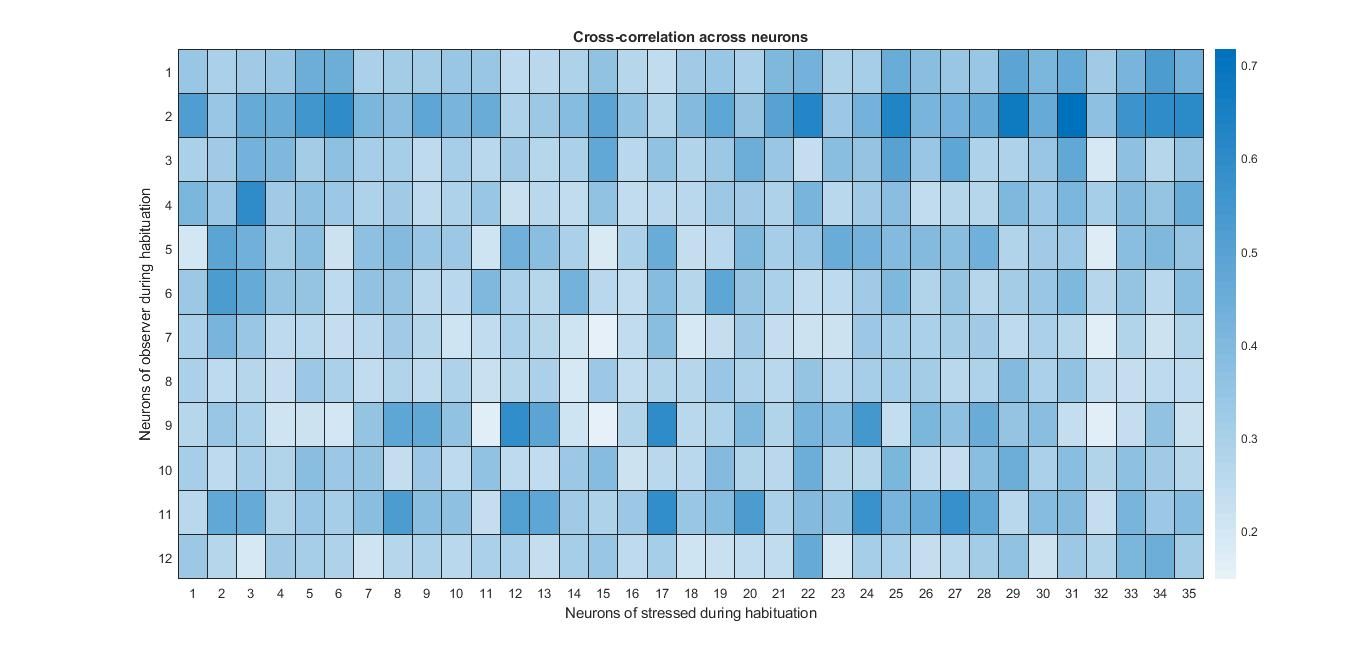
\includegraphics[scale=.30]{cc_heatmap2.jpg} 
	\end{center}  
	
	
\end{figure}


\end{frame}	




\begin{frame}
\frametitle{Neuron pairs synchronization: observer vs stressed during habituation (2)}


Fraction of pairs showing correlation = $1.66 \%$


\begin{figure}[H]
\begin{center}
	\hspace*{-1cm}
	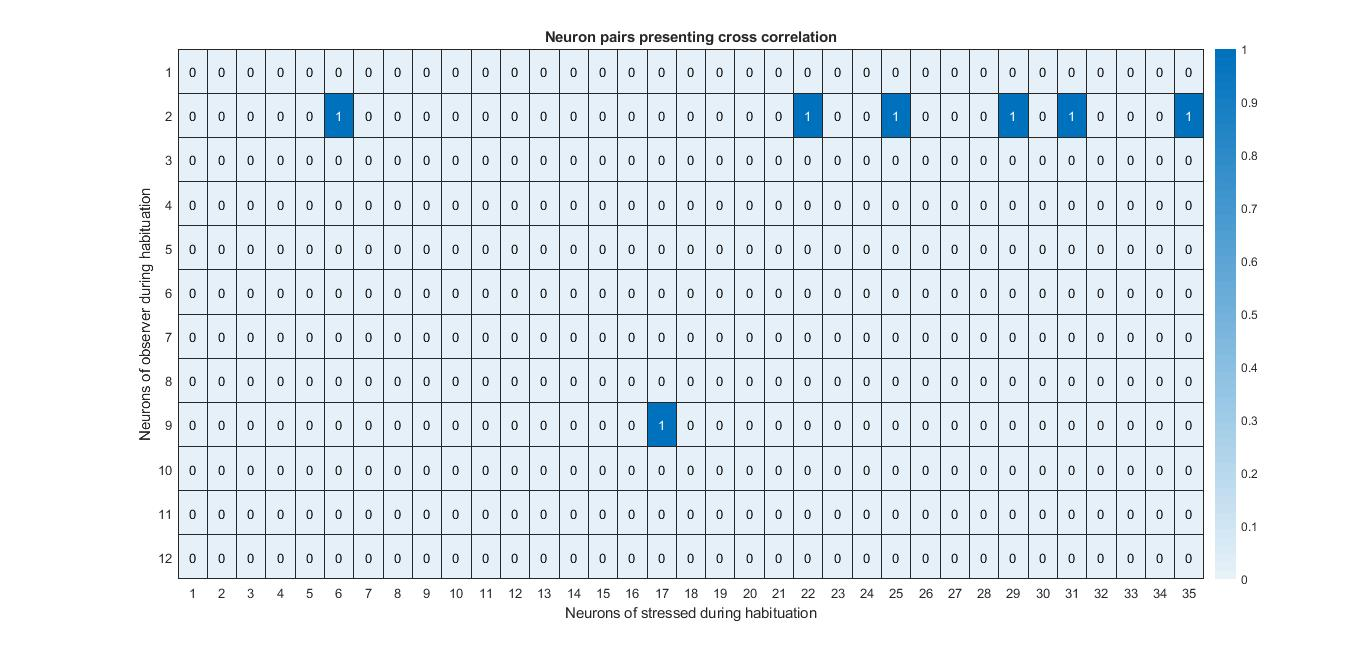
\includegraphics[scale=.30]{cc_active2.jpg} 
\end{center}  


\end{figure}


\end{frame}	


\begin{frame}
\frametitle{Neuron pairs synchronization: observer vs neutral during test (1)}





\begin{figure}[H]
	\begin{center}
		\hspace*{-1cm}
		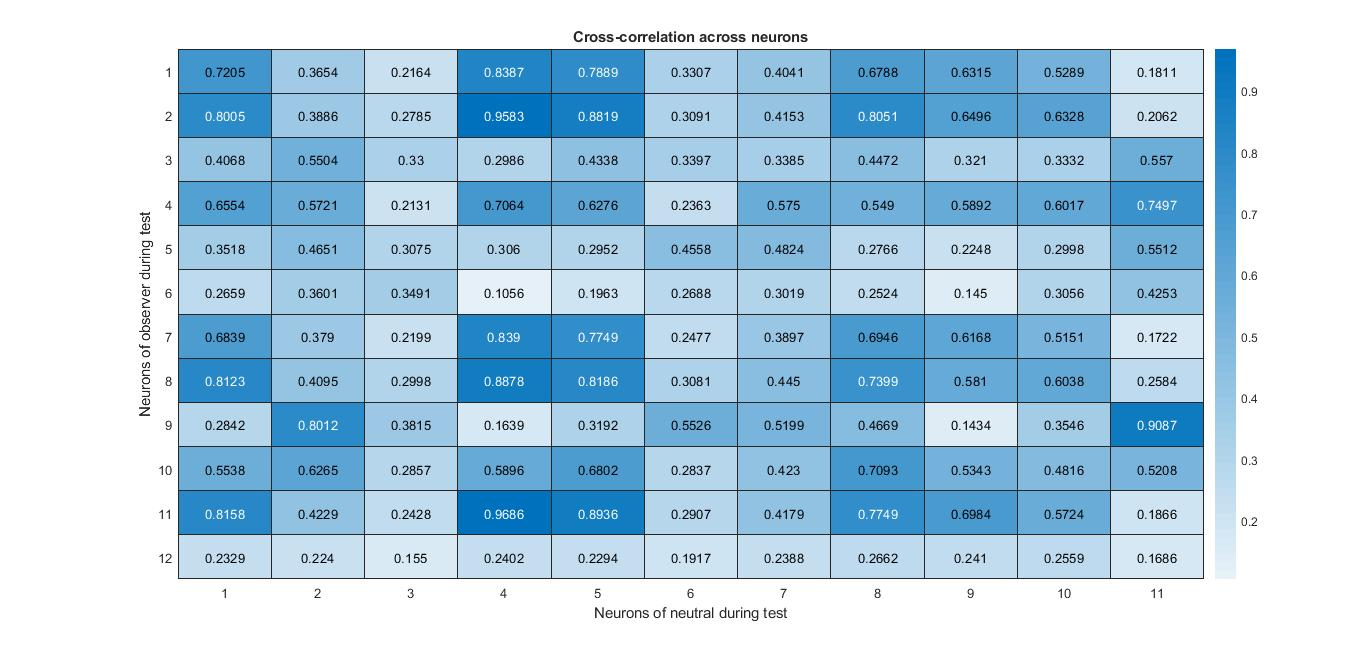
\includegraphics[scale=.30]{cc_heatmap3.jpg} 
	\end{center}  
	
	
\end{figure}


\end{frame}	




\begin{frame}
\frametitle{Neuron pairs synchronization: observer vs neutral during test (2)}


Fraction of pairs showing correlation = $23\%$


\begin{figure}[H]
\begin{center}
	\hspace*{-1cm}
	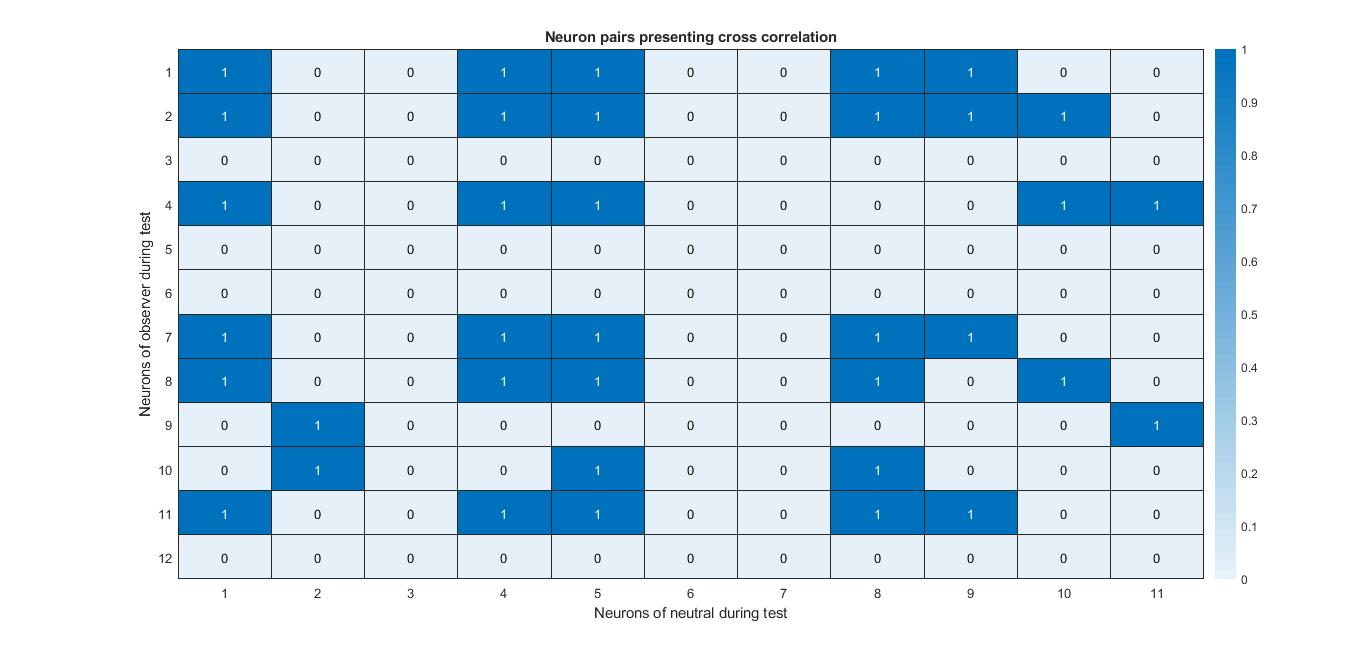
\includegraphics[scale=.30]{cc_active3.jpg} 
\end{center}  


\end{figure}


\end{frame}


\begin{frame}
\frametitle{Neuron pairs synchronization: observer vs neutral during habituation (1)}





\begin{figure}[H]
	\begin{center}
		\hspace*{-1cm}
		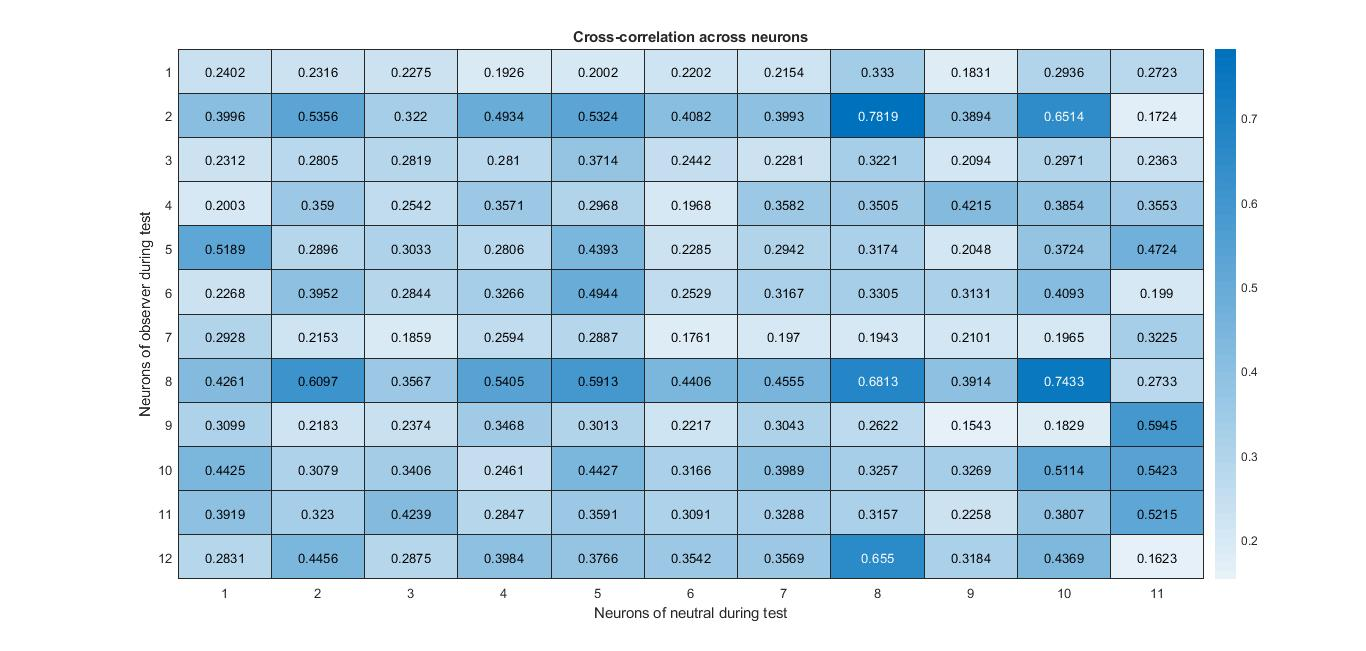
\includegraphics[scale=.30]{cc_heatmap4.jpg} 
	\end{center}  
	
	
\end{figure}


\end{frame}	




\begin{frame}
\frametitle{Neuron pairs synchronization: observer vs neutral during habituation (2)}


Fraction of pairs showing correlation = $4.5 \%$


\begin{figure}[H]
\begin{center}
	\hspace*{-1cm}
	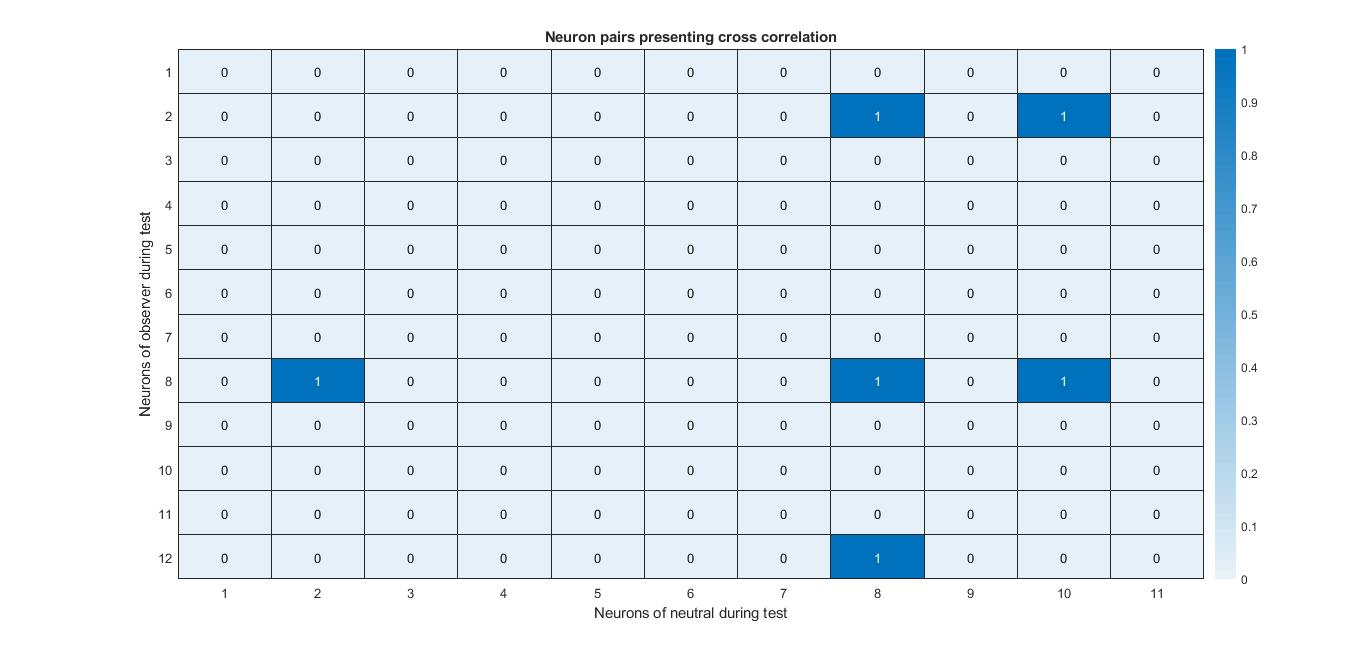
\includegraphics[scale=.30]{cc_active4.jpg} 
\end{center}  


\end{figure}


\end{frame}

\begin{frame}
\frametitle{Conclusions on the pairs correlation analysis}



\begin{itemize}
	
	\item For both the couples observer/stressed and observer/neutral, the fraction of neuronal pairs exhibiting correlation is higher during the test rather then the habituation 
	
	\item We can identify the neurons contributing the most to the correlation:\\
	Neurons $C00, C01, C03, C06, C07, C08, C09, C10$ for the observer \\
	Neurons $ C01, C02,  C07, C09, C11, C12, C17, C23, C24, C25$ for the stressed \\
	Neurons $C00, C01, C03, C04, C07, C08, C09, C10$ for the neutral 

	
	
	
\end{itemize}

\end{frame}	




\end{document}

\begin{frame}
\frametitle{}
\end{frame}